		\addtocontents{toc}{\vspace{0.1cm}}
		\subsection{Efecto de la amplitud de modulación a altas frecuencias}

				% Img:rateEquations
				\begin{figure}[H]
					\centering
					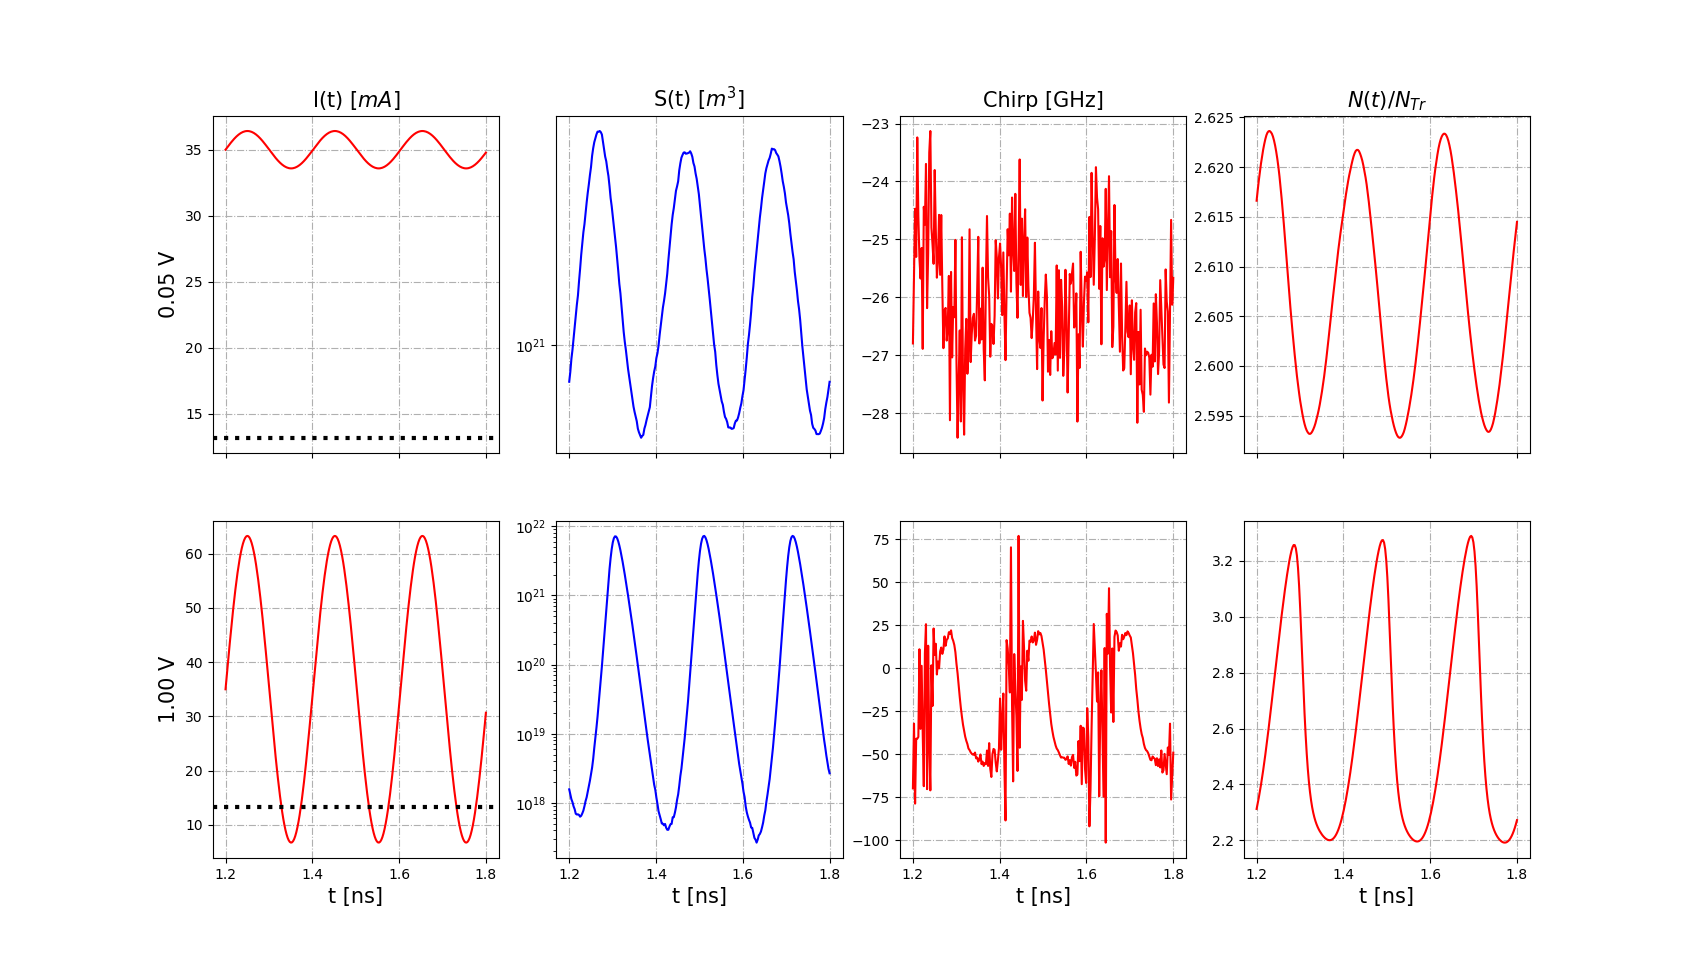
\includegraphics[width=1.0\linewidth]{rateEquations.png}
					\caption{\label{Img:rateEquations}RateEquations}	
				\end{figure}

				% Img:PSD
				\begin{figure}[H]
					\centering
					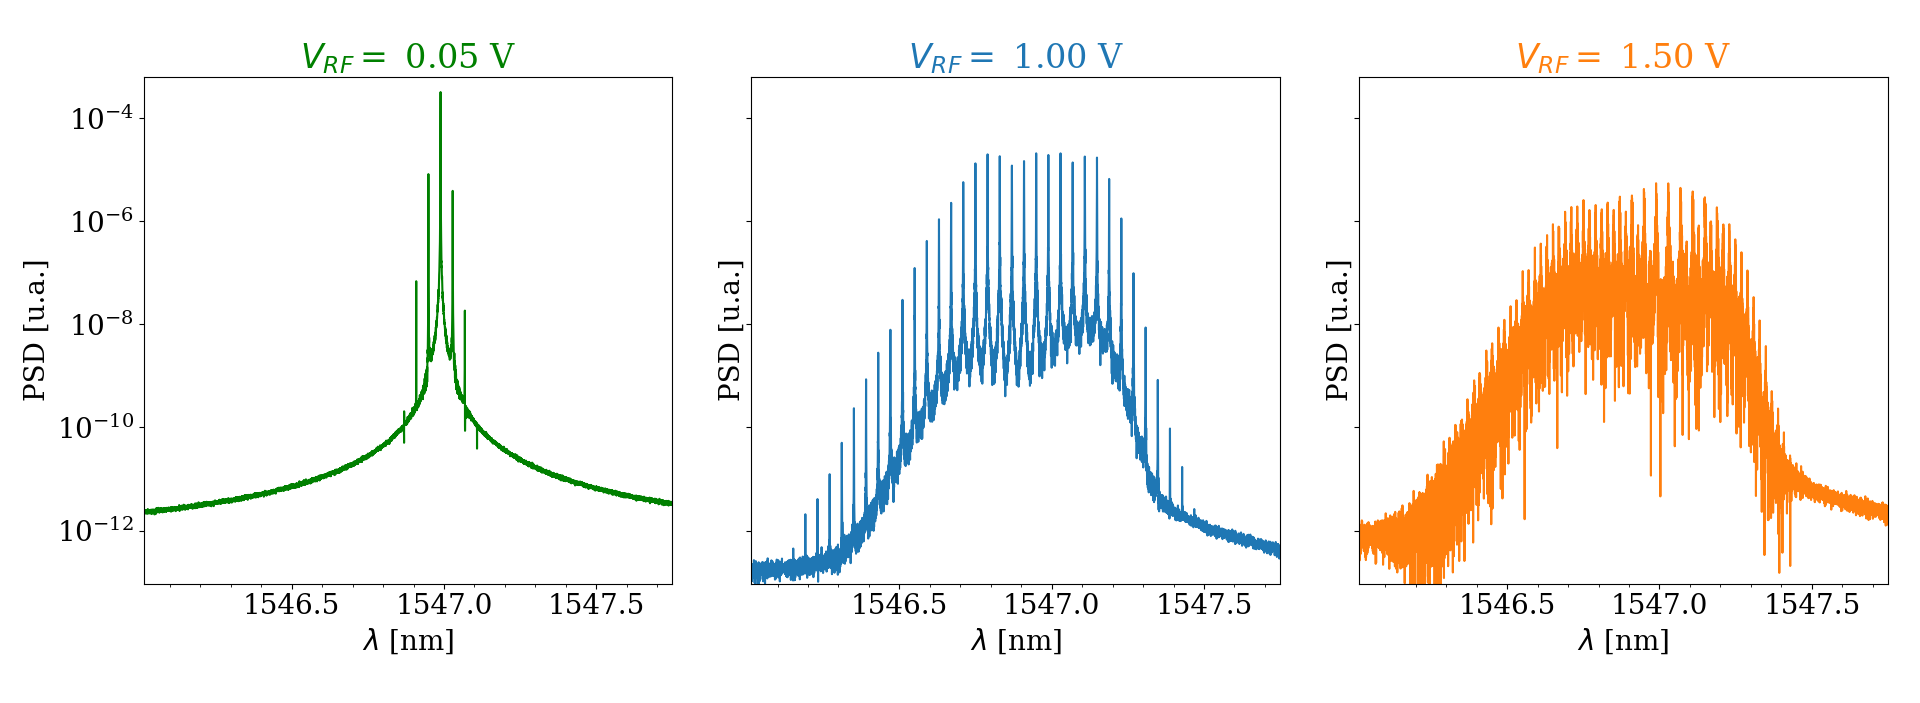
\includegraphics[width=1.0\linewidth]{PSD.png}
					\caption{\label{Img:PSD}PSD}	
				\end{figure}

				% Img:current
				\begin{figure}[H]
					\centering
					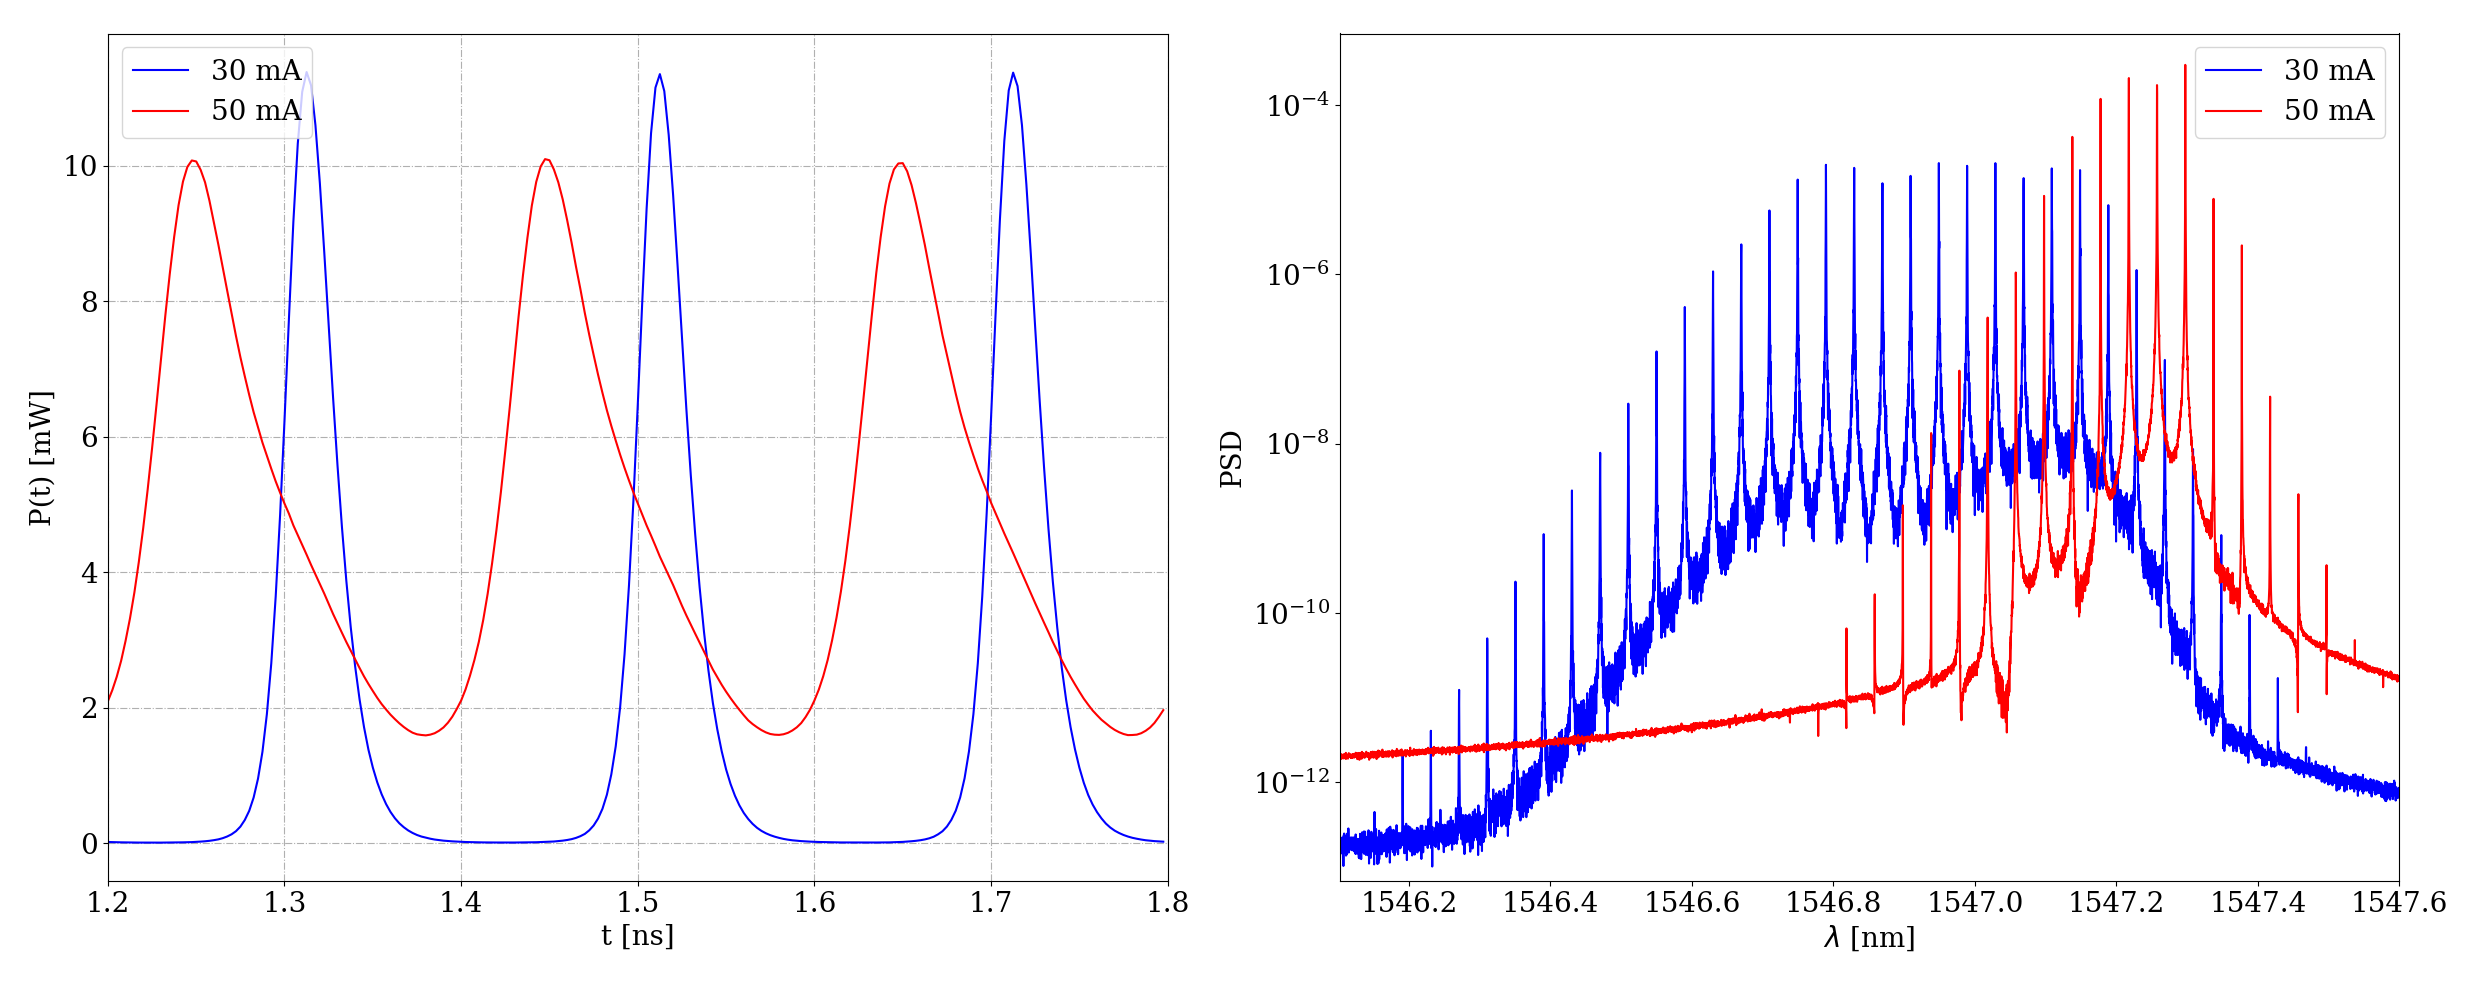
\includegraphics[width=1.0\linewidth]{current.png}
					\caption{\label{Img:current}Current}	
				\end{figure}

		\addtocontents{toc}{\vspace{0.1cm}}
		\subsection{Efecto de la amplitud de modulación a bajas frecuencias}

				% Img:500
				\begin{figure}[H]
					\centering
					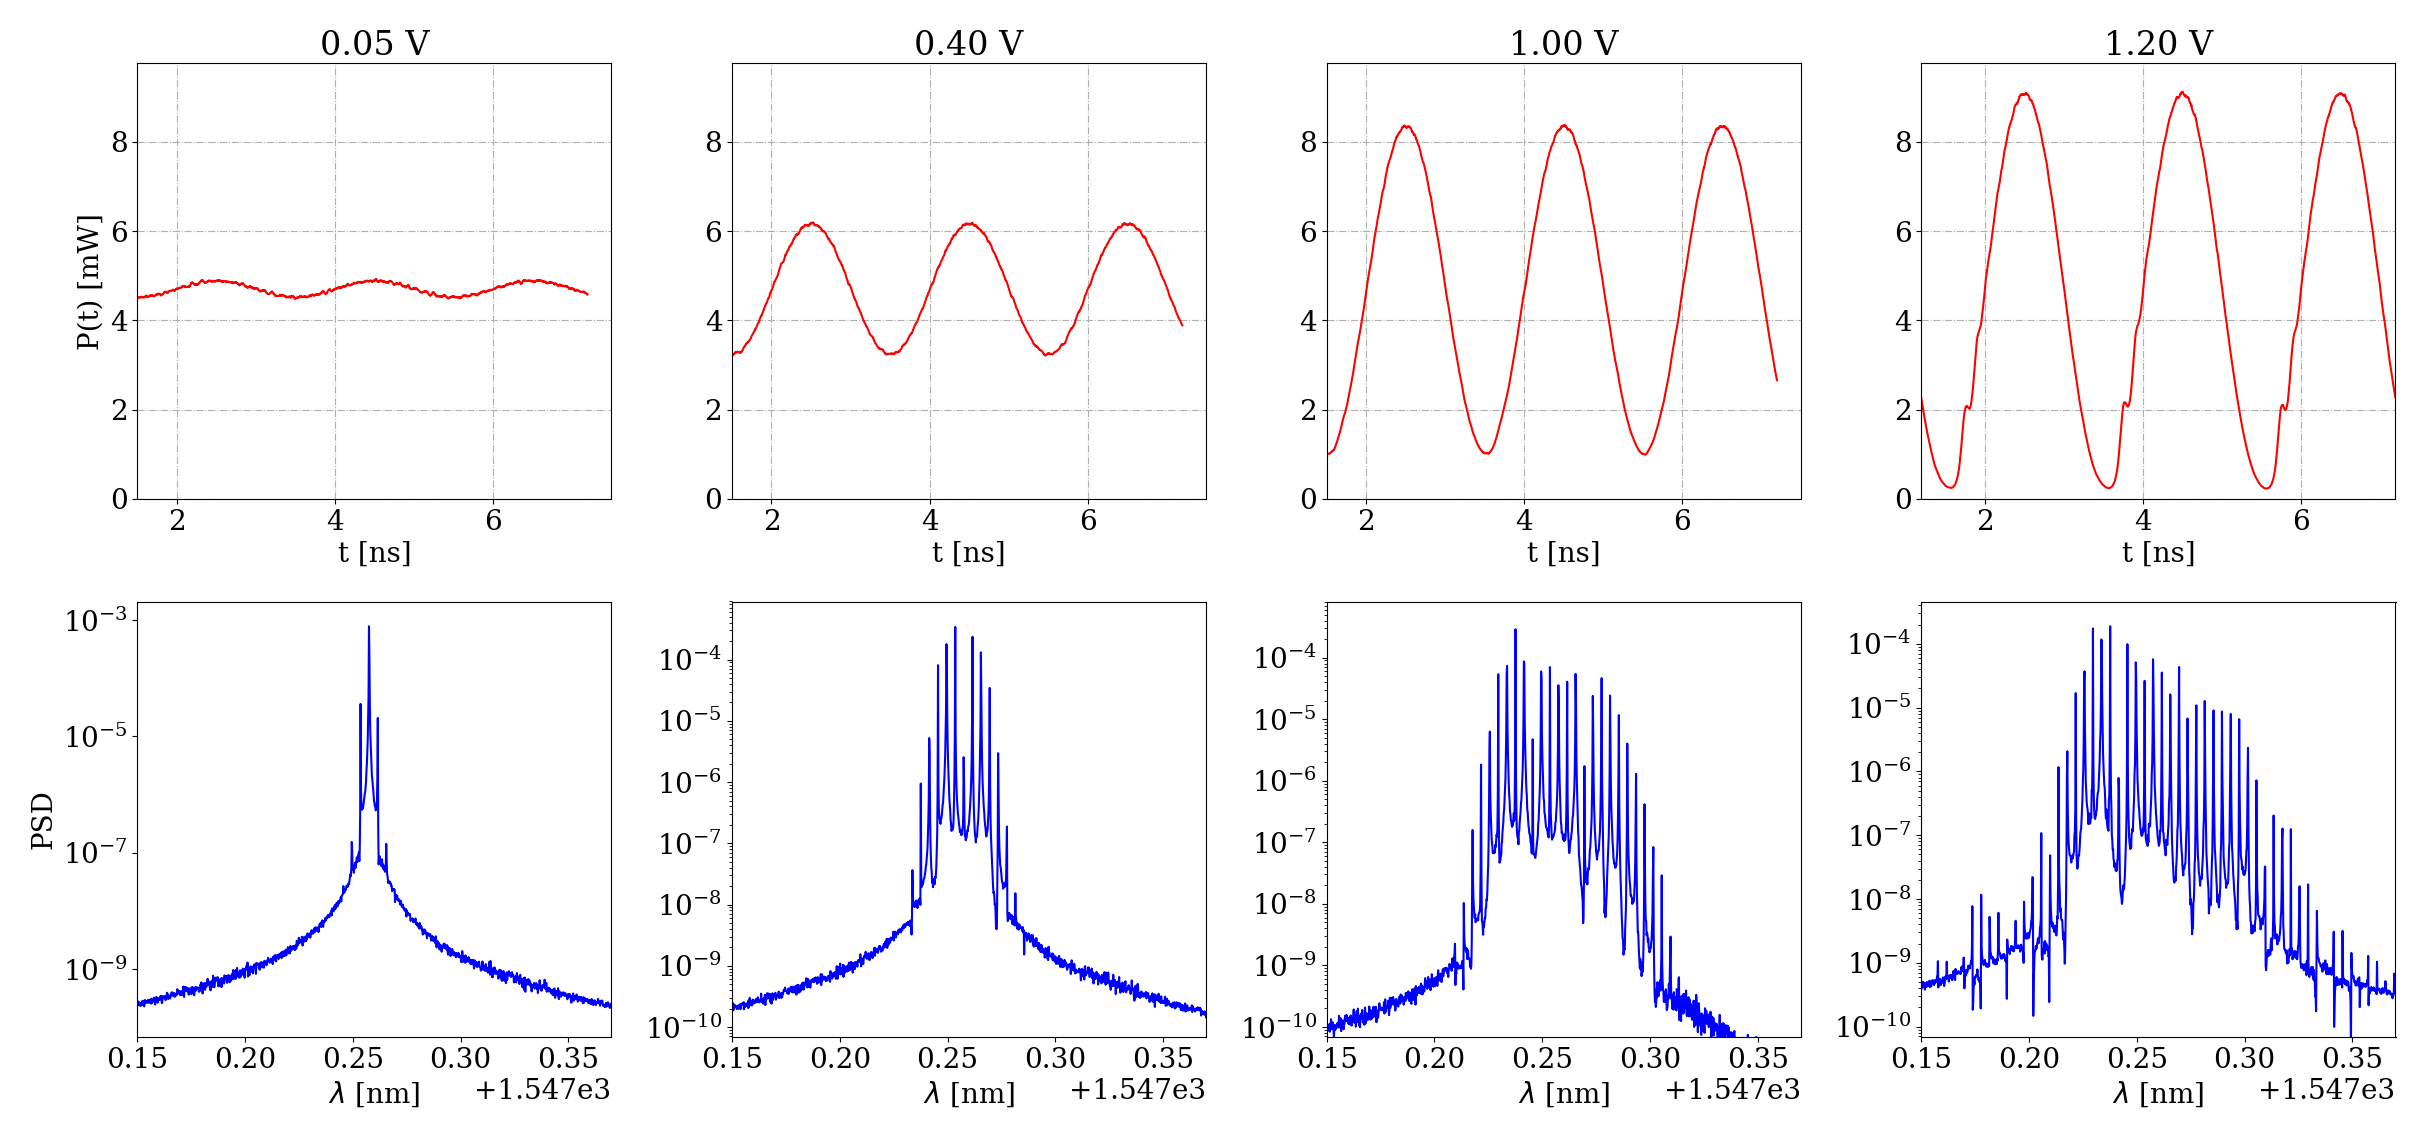
\includegraphics[width=1.0\linewidth]{500.png}
					\caption{\label{Img:500}500}	
				\end{figure}

				% Img:500mhz
				\begin{figure}[H]
					\centering
					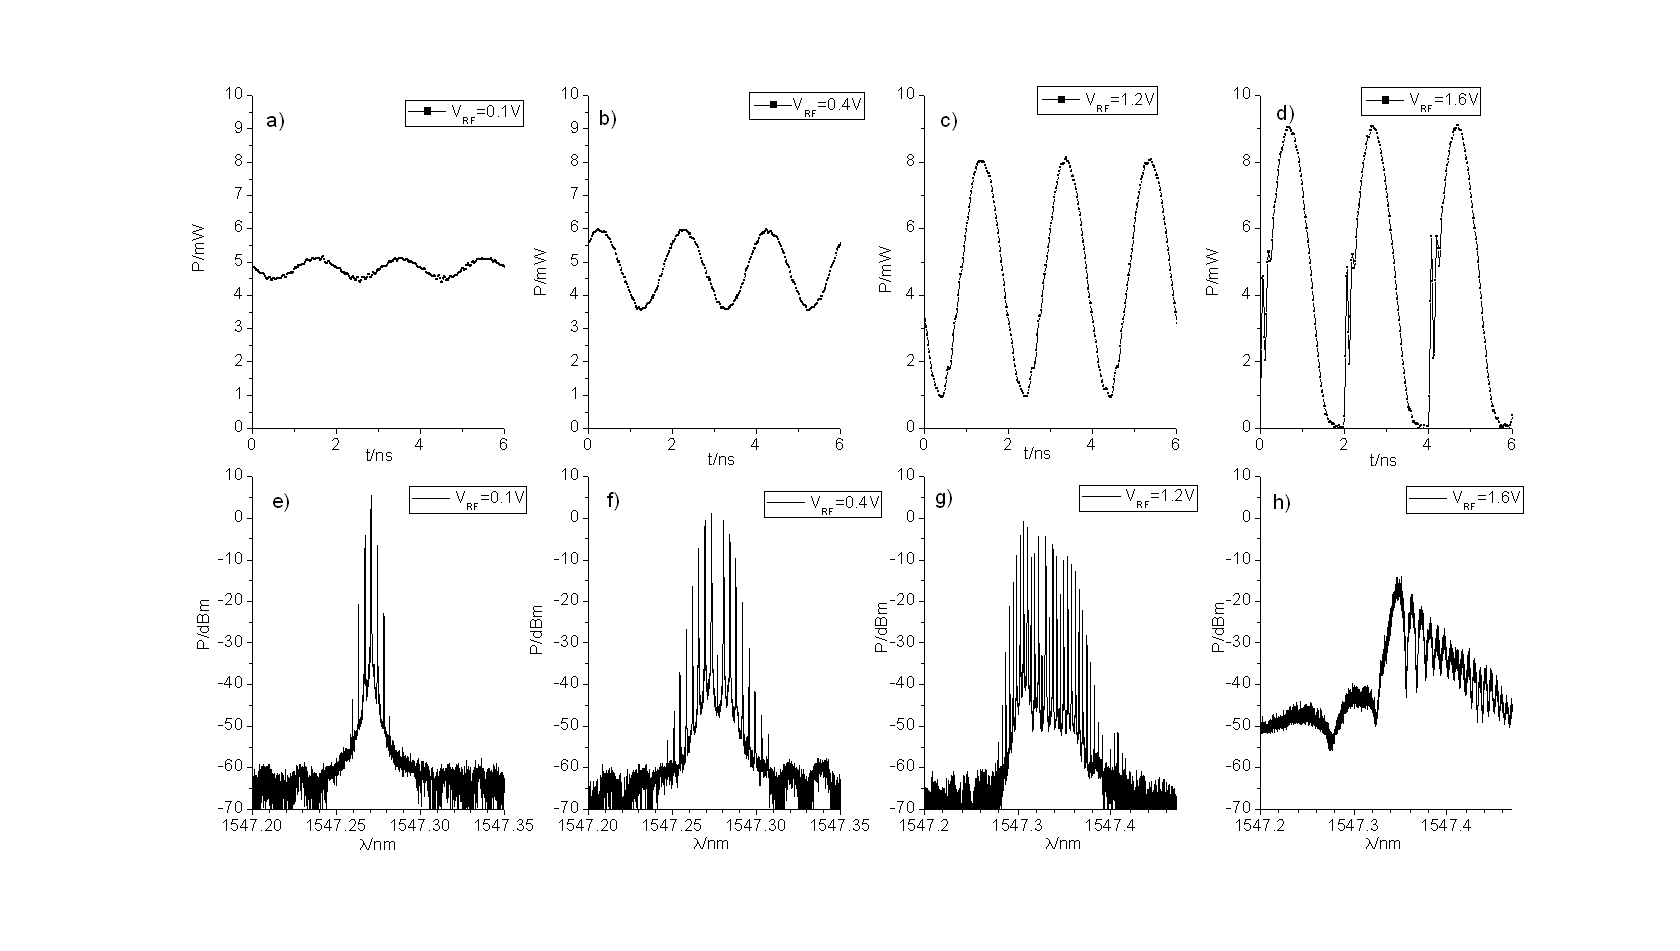
\includegraphics[width=1.0\linewidth]{../Chaves/OFC-GS/500mhz.png}
					\caption{\label{Img:500mhz}500mhz}	
				\end{figure}
